
% Chapter 04
% !TEX encoding = UTF-8 Unicode
\chapter{Parent-of-Origin Effects on Gene Expression }\label{ch:poeqtl}
\section[Abstract]{Abstract}

In this chapter, I explore the impact of parental origin of genetic variation on gene expression. We are interested in identifying any variants that are eQTLs but differ in direction by the parent the variant was inherited from. We performed opposite effect eQTL (oeQTL) and \emph{cis} maternal and paternal eQTL (mat-eQTL, pat-eQTL) using lymphoblastoid cell line (LCL) gene expression in 306 Hutterites. We did not find any variants that have opposite effects by parental origin on gene expression with either of these two approaches. We also used a $\chi^2$ test to search for parent specific effects on reciprocal heterozygotes using parent specific gene expression and identified SNPs that have modest parent-of-origin eQTL effects that need to be investigated further.

\section{Introduction}\label{ch04-introduction}
Imprinted genes have one allele silenced in a parent-of-origin specific manner. In humans, approximately 150 imprinted loci have been identified, many of which play important roles in development and growth \citep{Falls1999,Peters2014,Benonisdottir:2016dz}. Dysregulation of imprinted genes or regions can cause diseases that show parent-of-origin effects, such as Prader-Willi or Angelman syndrome, among others \cite{Peters2014}. Dysregulation of imprinted genes can be caused by large deletions but also by single variant mutations. Imprinted regions have also been associated with complex traits, such as height and age of menarche \citep{Benonisdottir:2016dz,Zoledziewska:2015do}, as well as common diseases such as obesity and some cancers \citep{Peters2014}. We know that SNPs associated with traits are more likely to be eQTLs \citep{Nicolae2010}, and here we explore if different parentally inherited alleles can have different impacts on gene expression and can be identified as parent-of-origin eQTLs with potential impacts on traits. We are not the first to look for parent-of-origin effects on gene expression: Garg et al. used gene expression in LCLs from HapMap trios to identify thirty imprinting eQTLs with parent-of-origin specific effects on expression of which two were known imprinted genes \citep{Garg2012a}. Garg et al. looked for impact of parent-of-origin specific effects on gene expression \citep{Garg2012a}, but no one has yet looked for eQTLs on parent specific expression coming from the same haplotype as the parentally inherited allele. 
	
Using RNA-seq and allele specific expression (ASE) we can map genes to parental haplotypes that will inform us of gene expression from parental chromosomes. With parentally mapped gene expression data, we can ask if genetic variation on the parental haplotype can influence gene expression from the same haplotype.  We are the first to look for 1) parental genetic variation that can have opposite effects on gene expression, as well as 2) maternal or paternally inherited genetic variation that could affect parental gene expression on the same chromosome. 	

We use methods to detect opposite parent-of-origin effects on total expression, as well as parent-specific expression in the Hutterites, a founder population of European descent, for which we have phased genotype data \cite{Livne2015}. We use RNA-seq from LCLs to map transcripts to parental haplotypes and use the parental gene expression to look for variation in \emph{cis} that would effect gene expression. Our study is likely underpowered to identify any opposite effect parent-of-origin eQTLs but we do identify a few parent-of-origin eQTLs where parentally inherited variation affects parent specific gene expression from the same haplotype. There is no known biological mechanism as to why parent-of-origin eQTLs could exist outside of imprinted loci.

\section{Results}\label{ch04-results}

For each of 306 individuals, the total number of transcripts at each gene was assigned as maternally inherited, paternally inherited, or unknown parent of origin. The last group included transcripts without heterozygote SNPs or SNPs without parent-of-origin information. Transcripts were assigned to the parentally inherited categories using SNPs in the reads and matching alleles to either the known maternally or paternally inherited alleles. All the genes analyzed had some transcripts of unknown origin (average 97.8\%, range 8.3-100\%). For each gene we assigned parental origin to an average of 1.8\% of transcripts (range: 0-34.7\%), and for each individual we assigned parental origin to an average of 1.4\% of transcripts (range: 0-1.7\%). On average, about 40 SNPs per gene were used to assign the transcripts of a gene to a parent (range 1-1839 SNPs). 


\subsection{Opposite Parent-of-Origin eQTL (oeQTL) }\label{Opposite Parent-of-Origin eQTL (oeQTL)} 
Our original oeQTL identified three significant opposite effect associations but these associations were driven by one individual's genotype. The significant associations are shown in Figures \ref{fig:oeQTL}. Once we subset SNPs on having at least three individuals in each of three genotype groups, we did not find any significant results (Bonferroni corrected p-value). 

\begin{figure}[!htb]
\centering 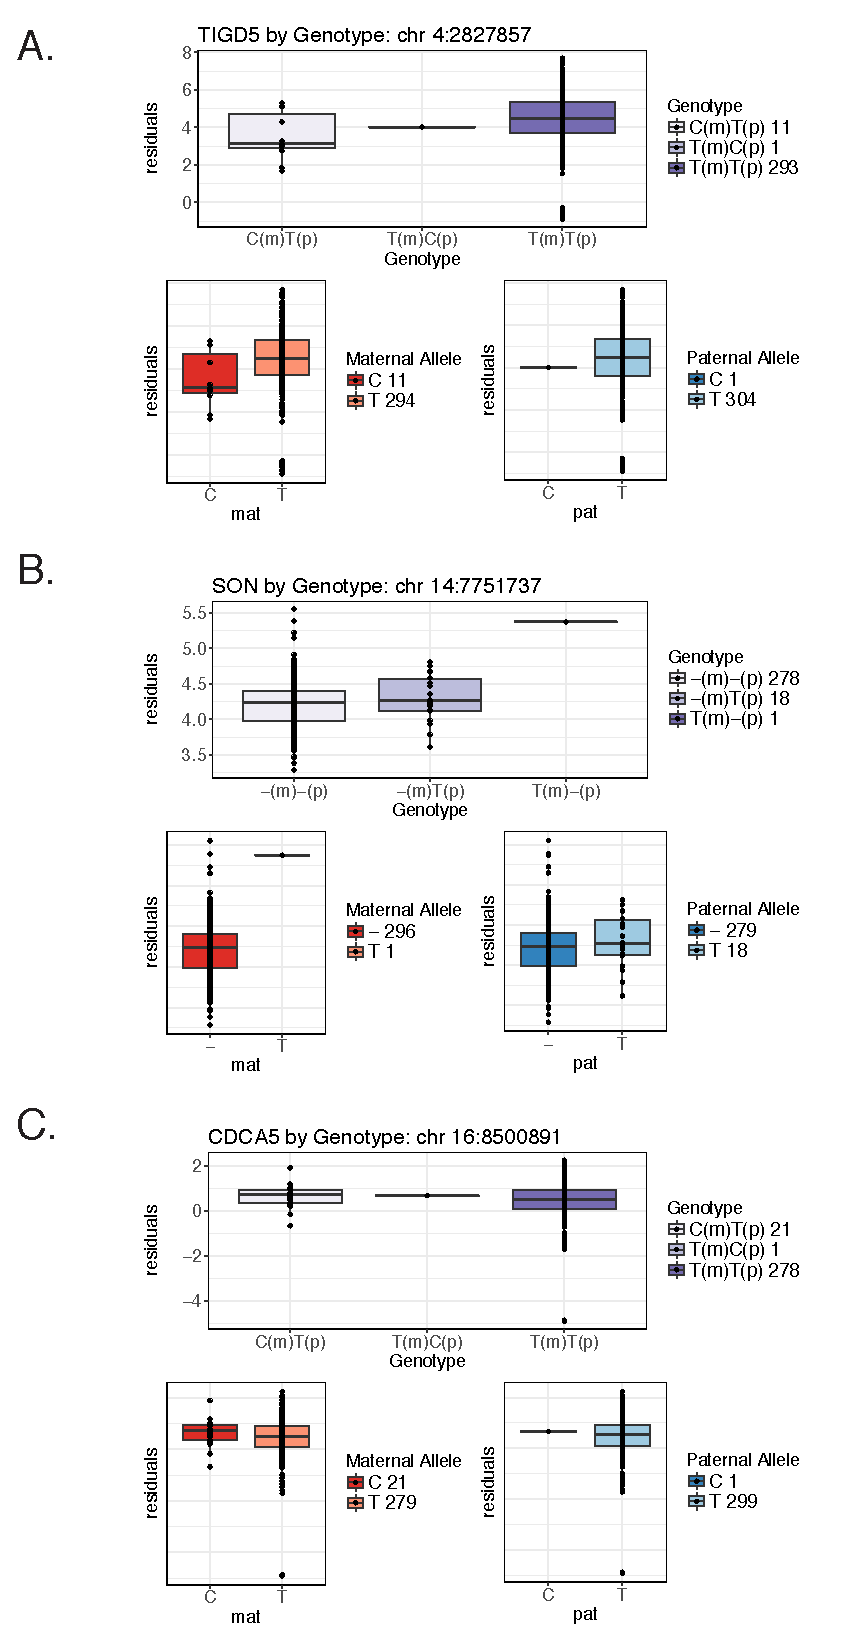
\includegraphics[width=4in]{img/ch04/fig-01-oeQTLs.pdf}
\caption[Opposite effect eQTLs driven by one individual's genotype.]{\textbf{Opposite effect eQTLs driven by one individual's genotype.} The three most significant opposite effect eQTLs for genes A) \emph{TIGD5} (p-value $ 3.1 \times 10^{-9} $), B) \emph{SON} (p-value $4.3 \times 10^{-9} $) and C) \emph{CDCA5} (p-value $3.5 \times 10^{-9} $). The parent-of-origin eQTL is driven by one heterozygous individual for each gene.}
\label{fig:oeQTL}
\end{figure}
\clearpage

\subsection{Single Parent eQTL (mat-eQTL, pat-eQTL)}\label{Single Parent eQTL (mat-eQTL, pat-eQTL)} 
We performed the mat-eQTL and pat-eQTL analysis, using parent-of-origin normalized expression. We normalized the parental gene expression data using library sizes from the total gene expression(see Methods). However, the data was sparse and zeros drove most of the analysis. The significant maternal and paternal associations were driven by zeros in the data shown in Figures \ref{fig:mat-eQTL} and \ref{fig:pat-eQTL}. 

\begin{figure}[!htb]
\centering 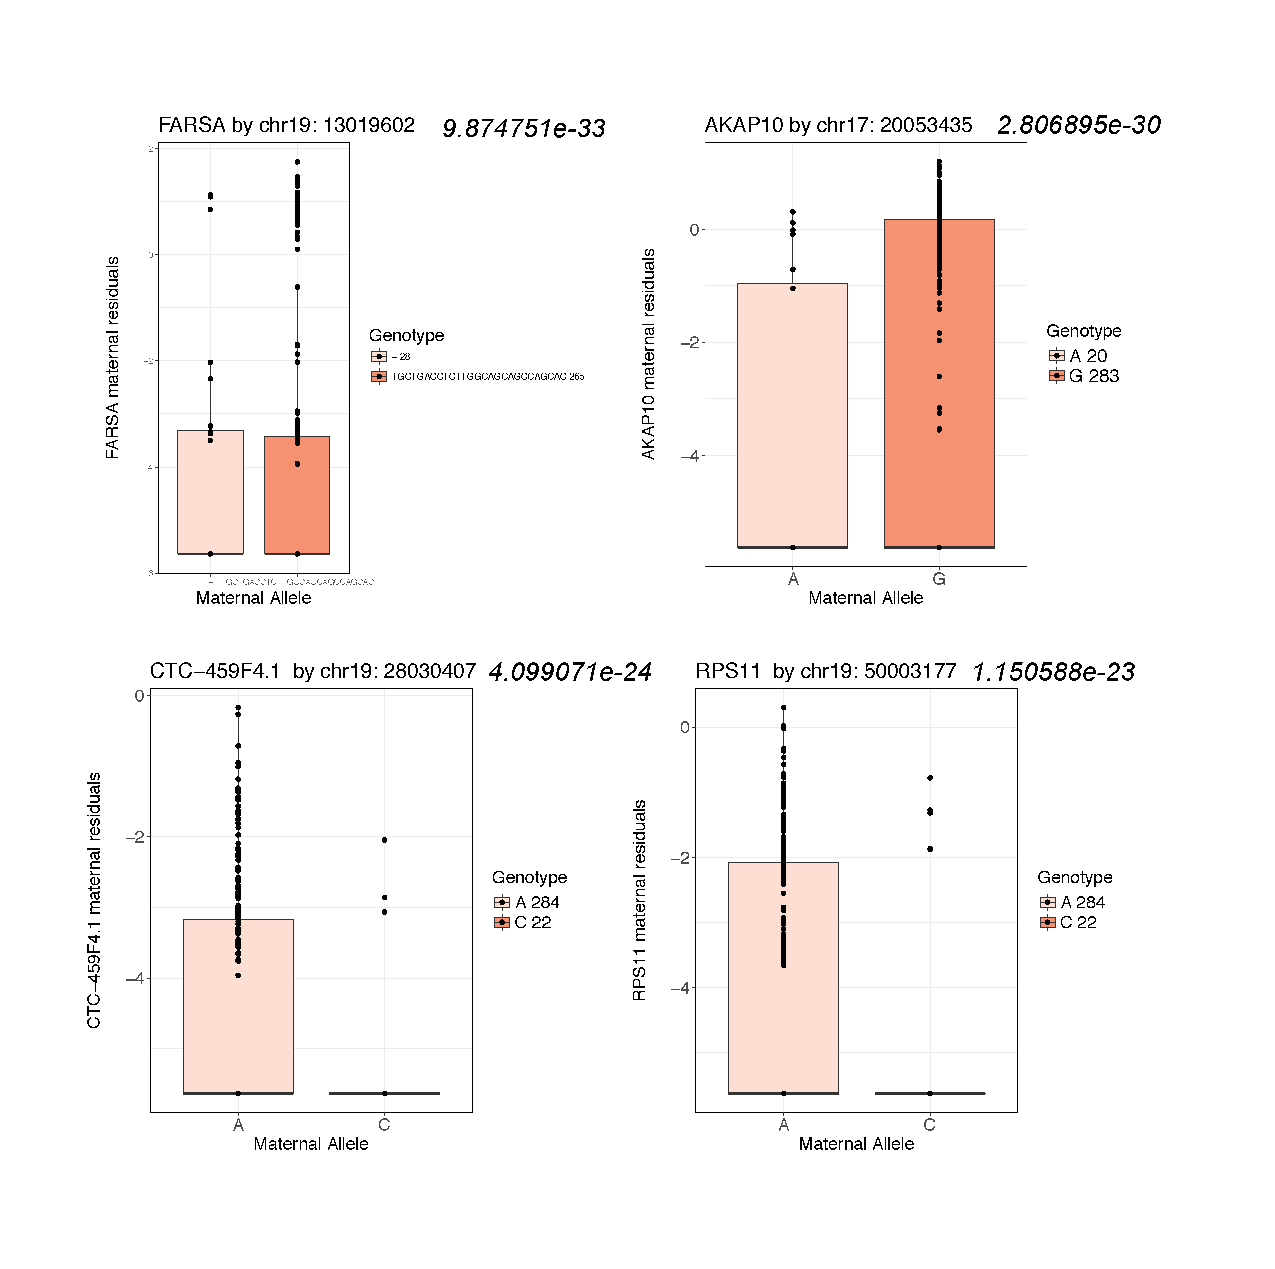
\includegraphics[width=4in]{img/ch04/fig-04-mat-eQTL.pdf}
\caption[Maternal eQTL Associations Driven by Null Values.]{\textbf{Maternal eQTL Associations Driven by Null Values.} The four most significant maternal eQTL associations. Most of the individuals have no value of expression for these genes, we see most of the genes have a median that corresponds to a value of zero after normalization. }
\label{fig:mat-eQTL}
\end{figure}

\begin{figure}[!htb]
\centering 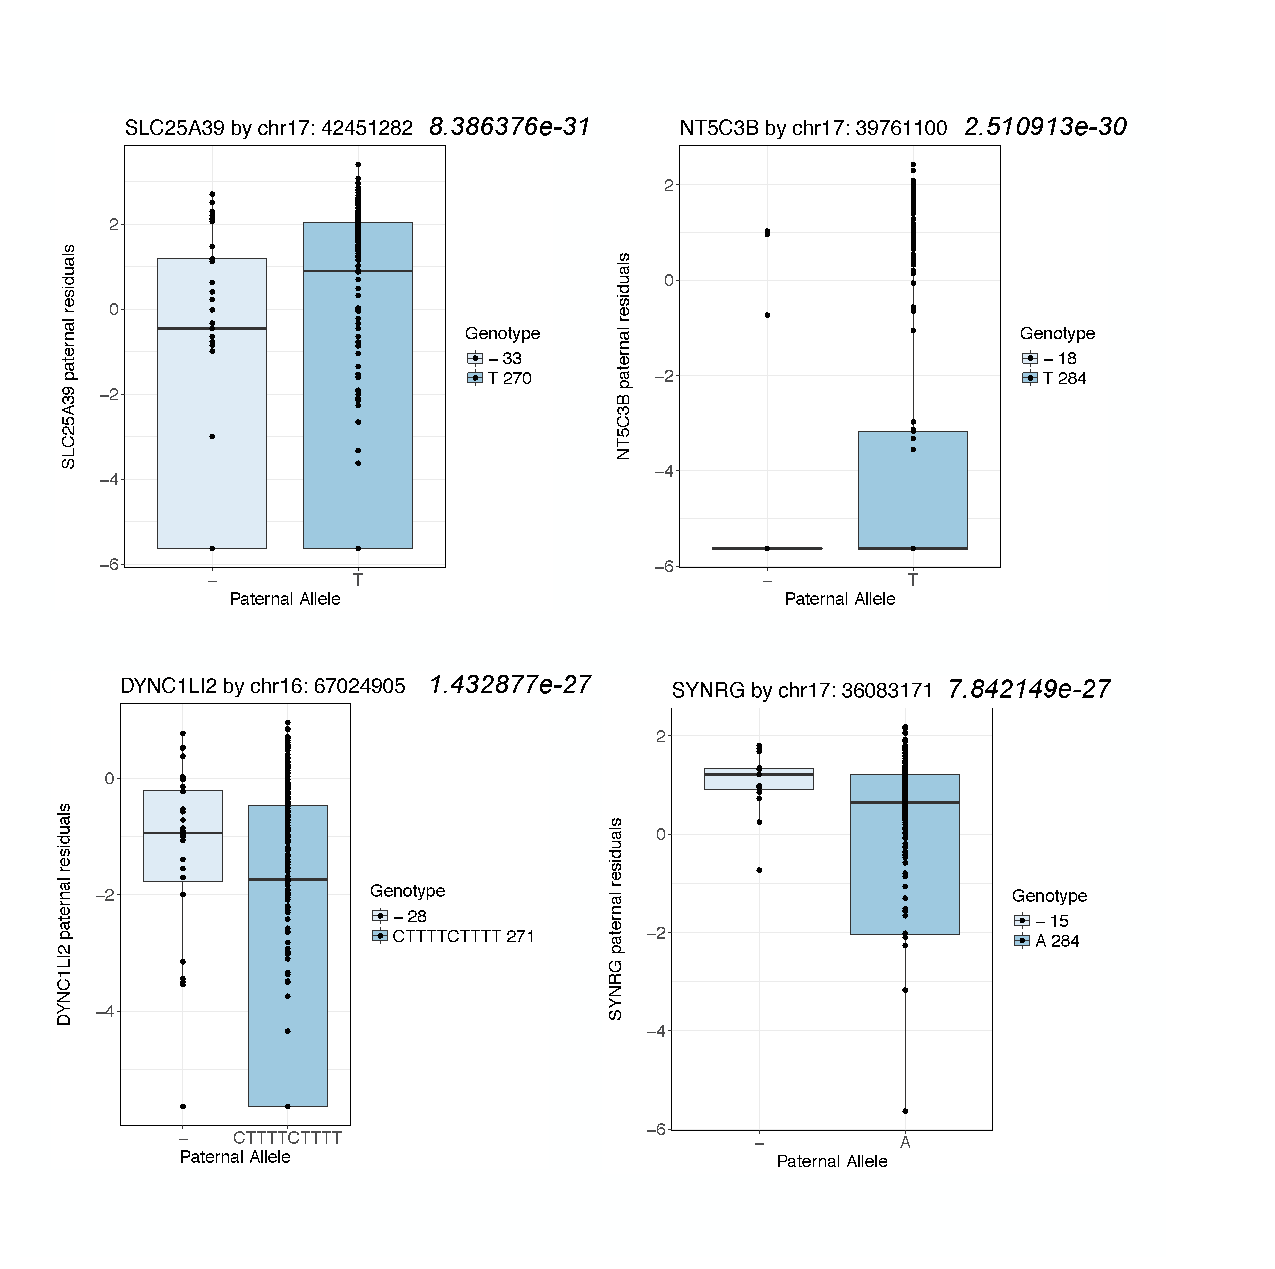
\includegraphics[width=4in]{img/ch04/fig-05-pat-eQTL.pdf}
\caption[Paternal eQTL Associations Driven by Null Values.]{\textbf{Paternal eQTL Associations Driven by Null Values.} The four most significant paternal eQTL associations. Most of the individuals have no value of expression for these genes, we see most of the genes have a median that corresponds to a value of zero after normalization. }
\label{fig:pat-eQTL}
\end{figure}


To address this problem, we redid the same analysis using only informative reads, removing zeros that were due to absence of heterozygous SNPs in the gene (see Methods for more detail). There were 7,398,096 SNP-gene pairs we could compare across both single parent eQTLs. For eQTLs significant in both, (60,549 SNP gene pairs), the effect sizes were all in the same direction: no SNPs had opposite effects on their corresponding parental gene expression (Figure \ref{fig:effectsizes}). The imbalance of positive and negative effect sizes in Figure \ref{fig:effectsizes} is likely due in large part to the sparsity of the data, where most individuals have an expression value of zero and any individuals with some measure of expression drive the effect size to be positive.

\begin{figure}[!htb]
\centering 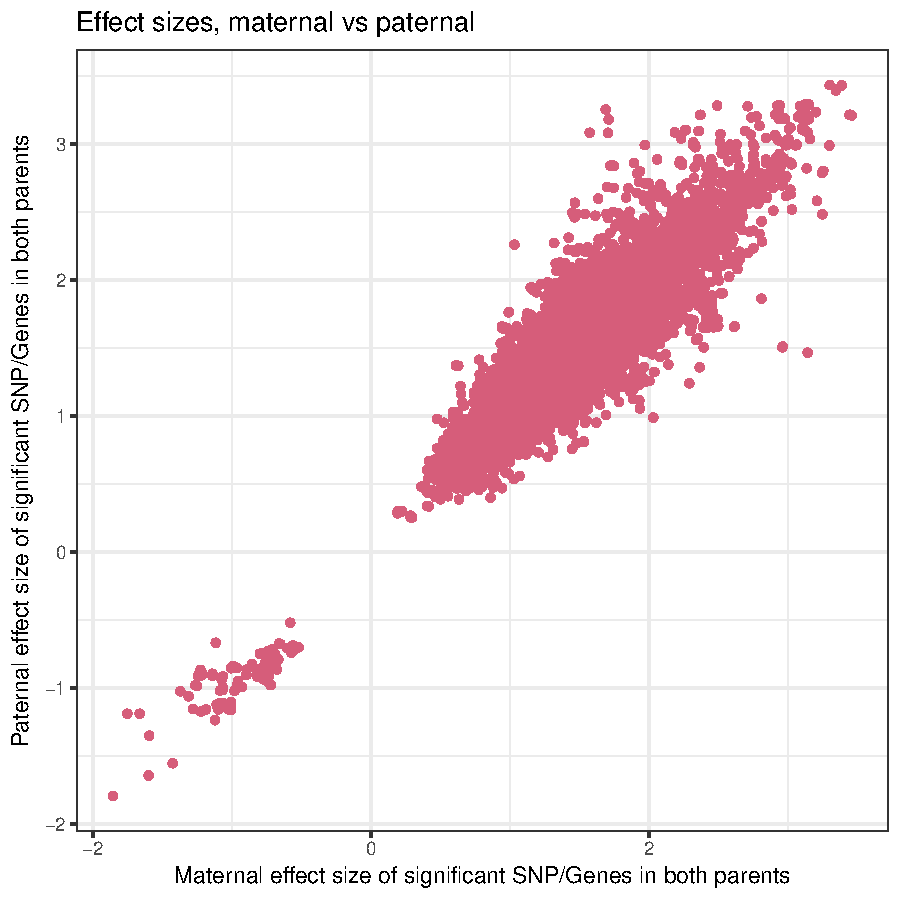
\includegraphics[width=4in]{img/ch04/fig-06-effectsizes.pdf}
\caption[Similar effect sizes across mat-eQTL and pat-eQTL.]{\textbf{Similar effect sizes across mat-eQTL and pat-eQTL.} }
\label{fig:effectsizes}
\end{figure}


We compared SNP gene pairs that were significant (Bonferroni) in one parent, and not significant (p \textgreater 0.05) in the other parent. 7,712 SNP-gene pairs were maternally significant and not paternally significant and 10,815 paternal significant associations were not maternally significant. An example of each is shown in Figure \ref{fig:sig_notsig} where the maternally inherited A allele at 20:20036897 in Figure \ref{fig:sig_notsig}A is associated with increased maternal expression, but at least half of the individuals with the paternally inherited A allele at the same SNP have no expression from the paternal haplotype. In Figure \ref{fig:sig_notsig} B, the A allele at 9:134850002 is associated with increased paternal expression when inherited from the father but not when inherited from the mother.


\begin{figure}[!htb]
\centering 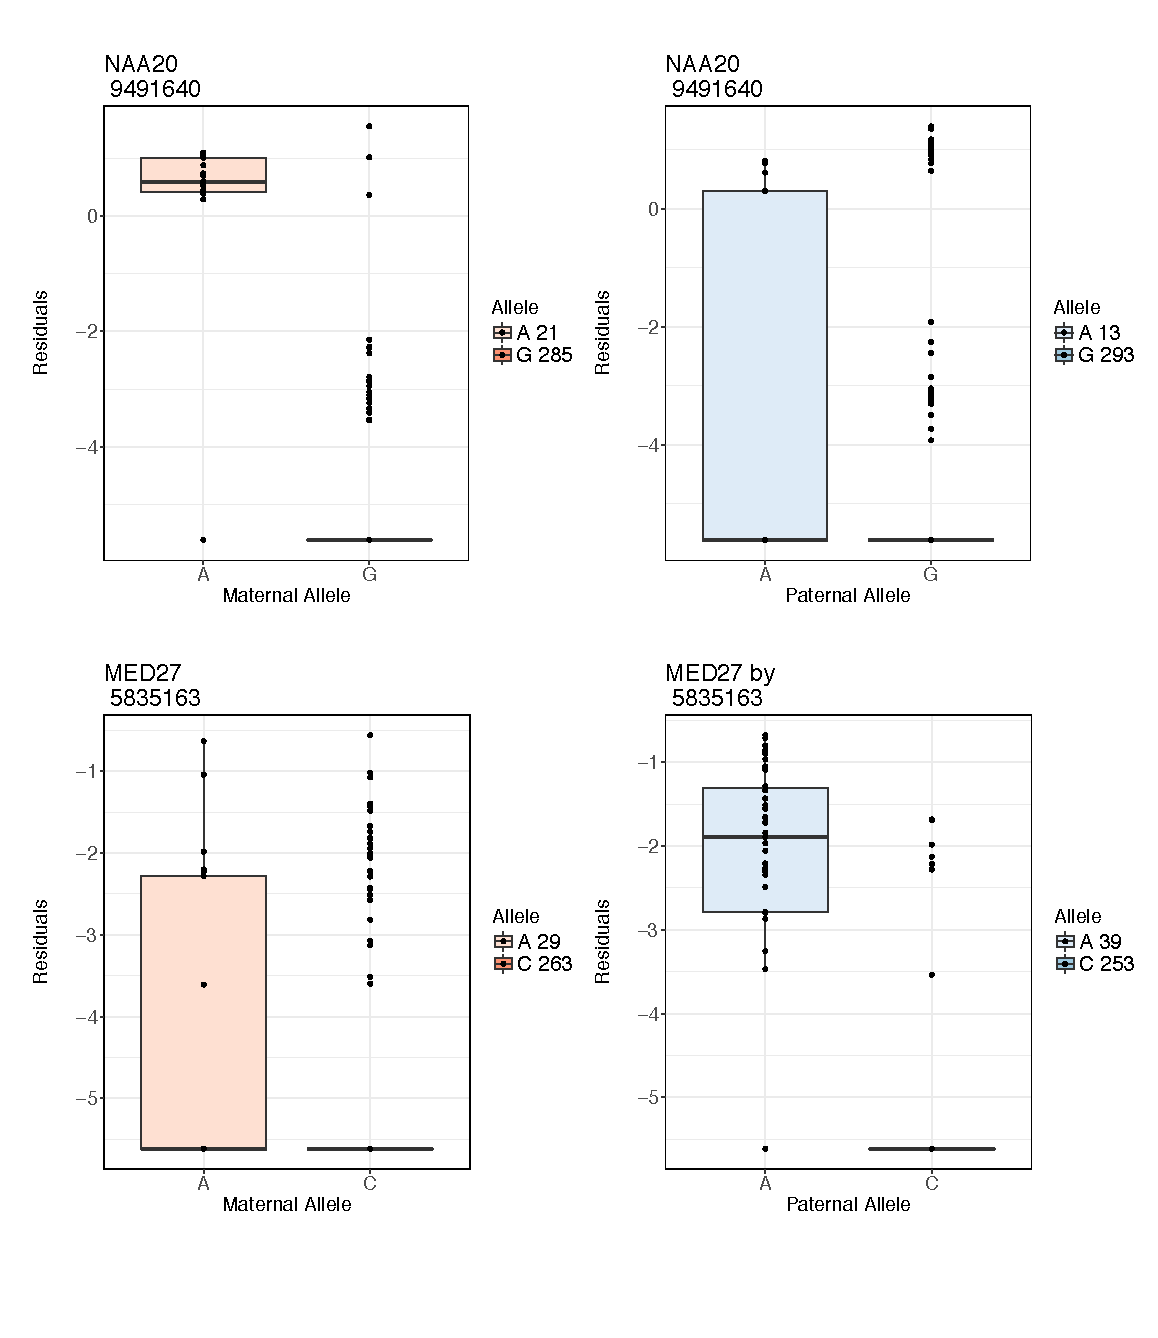
\includegraphics[width=5in]{img/ch04/fig-07-sig_notsig.pdf}
\caption[Parent specific eQTLs significant in one parent and not the other.]{\textbf{Parent specific eQTLs significant in one parent and not the other.} (A) Variant on chromosome 20:20036897 has a significant mat-eQTL association (left) with gene \emph{NAA20} (p-value = $2.32 \times 10^{-27} $) where the pat-eQTL (right) from the same variant is not significant (p-value = $2.18 \times 10^{-2} $). In contrast, (B) Variant on chromosome 9:134850002 has a significant pat-eQTL association (right) with gene \emph{MED27} (p-value = $4.7 \times 10^{-32} $) and mat-eQTL is not significant (p-value = $2.75 \times 10^{-3} $) (left).}
\label{fig:sig_notsig}
\end{figure}


\subsection{Parent-of-Origin (PO) - ASE Test}\label{Parent-of-Origin (PO) - ASE Test} 

To detect parent-of-origin effects on expression using a different approach, we did a PO ASE test (see Methods) using parental gene expression count data. We identified 56,800 significant results using a Bonferroni corrected p-value . The top ten significant genes with their most significant SNPs are included in Table \ref{tab:poase1}. The top four genes with their most significant SNPs shown in Figures \ref{fig:SNHG14}, \ref{fig:ERAP2}, \ref{fig:ZDBF2}, and \ref{fig:PEG10}. Of the 10 most significant genes, 5 are imprinted (\emph{SNHG14}, \emph{ZDBF2}, \emph{PEG10}, \emph{L3MBTL1}, \emph{FAM50B}.)

\begin{table}[!htb]
\centering
\begin{adjustbox}{width={\textwidth}}
\begin{tabular}{@{}p{1cm}p{3cm}p{3cm}p{5cm}p{5cm}p{3cm}@{}}
 \toprule  Chr & bp & Gene & Maternal Reads (Ref/Alt) & Paternal Reads (Ref/Alt) & p-value \\ \midrule
15 & 8034579 & \emph{SNHG14}* & 15/11  & 587/983 & 0 \\
2 & 1459666  & \emph{ZDBF2}* & 34/49  & 638/1190 & 0\\
5 & 3342675 & \emph{ERAP2} & 3948/2445 & 4790/7067 & 0\\
7 & 4671649 &  \emph{PEG10}* & 42/4  & 635/1073 & 0 \\
8 & 5271050 & \emph{PABPC1} & 600/2564 & 21/494 & 0 \\
20 & 9548868 & \emph{L3MBTL1}* & 13/18 & 527/699 & 9.88E-248 \\
14 & 8007882 & \emph{IGHG1} &   794/156  & 1711/918 & 5.15E-191\\
6 & 3666034 & \emph{FAM50B}* & 0/6 & 481/362 & 1.58E-180\\
22 & 9799426 & \emph{IGLV2-5} & 240/499 & 23/1 & 6.56E-145\\
6 & 3758995 & \emph{BTN3A2} & 3609/1049  & 3328/3330 &  8.40E-144\\  \bottomrule
\end{tabular}
\end{adjustbox}
\caption[Top Ten Significant Genes from PO-ASE Test.]{\textbf{Top Ten Significant Genes from PO-ASE Test.} Five of the top ten significant genes from the PO-ASE test are imprinted genes (* represents imprinted genes). P-value of 0 corresponds to a really small p-value (\textless $10 \times 10^{-248} $)}
\label{tab:poase1}
\end{table}


\begin{figure}[!htb]
\centering 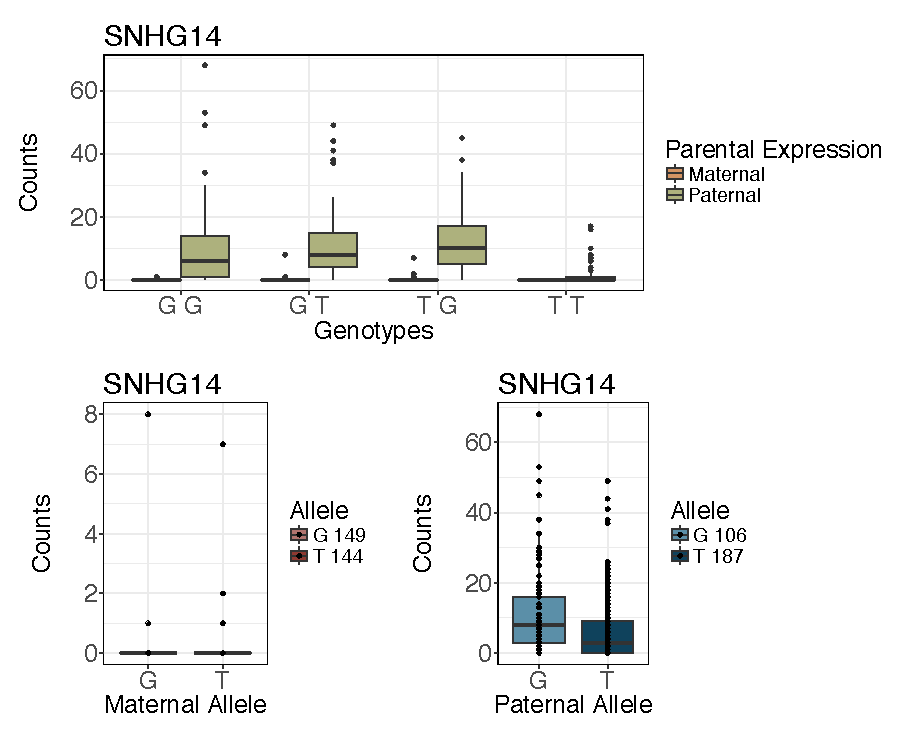
\includegraphics[width=3.5in]{img/ch04/SNHG14.pdf}
\caption[Significant PO-ASE association with gene \emph{SNHG14}.]{\textbf{Significant PO-ASE association with gene \emph{SNHG14}.} For imprinted gene \emph{SNHG14} we see variation in expression based on the allele and the parent it was inherited from. The paternally inherited T and G allele have different expression levels. Due to the imprinted status of the gene, we also see consistently more paternal expression from both alleles than maternal expression.}
\label{fig:SNHG14}
\end{figure}

\begin{figure}[!htb]
\centering 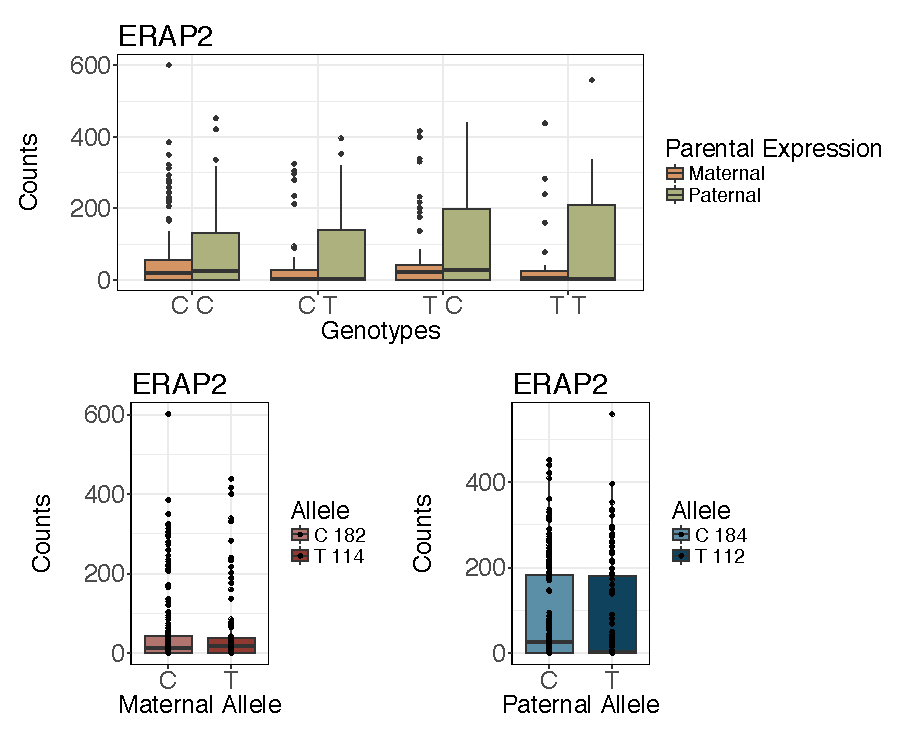
\includegraphics[width=3.5in]{img/ch04/ERAP2.pdf}
\caption[Significant PO-ASE association with gene \emph{ERAP2}.]{\textbf{Significant PO-ASE association with gene \emph{ERAP2}.} For gene \emph{ERAP2} Alleles C and T have different expression levels based on which parent the allele was inherited from. We see more expression form the paternal G allele than the paternal A allele in the reciprocal heterozygotes. Similar to imprinted genes, we see more paternal expression and less maternal expression across both alleles.  }
\label{fig:ERAP2}
\end{figure}


\begin{figure}[!htb]
\centering 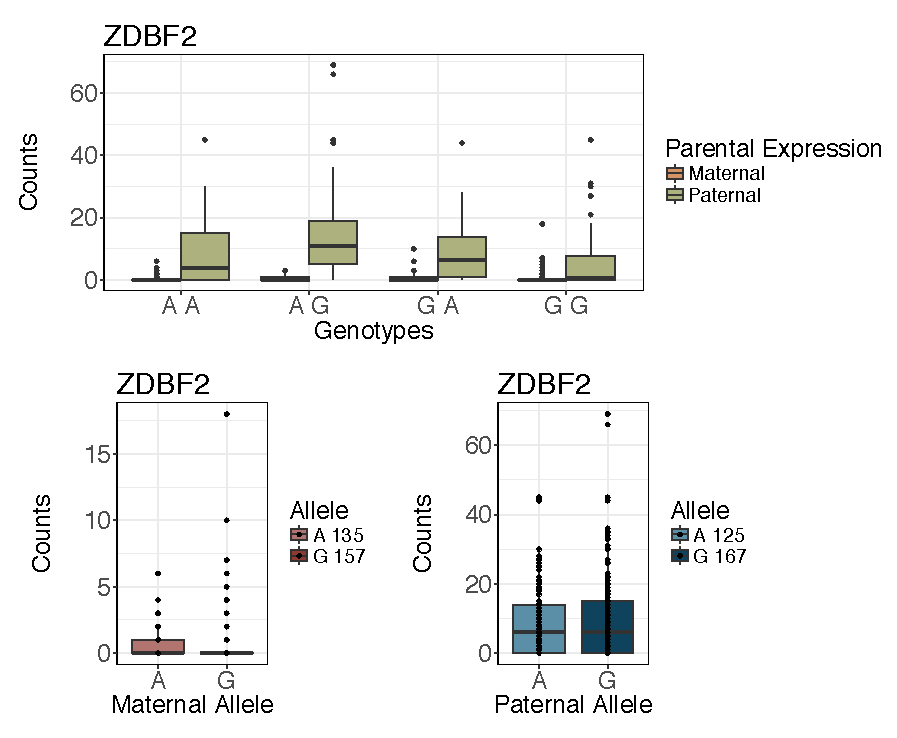
\includegraphics[width=3.5in]{img/ch04/ZDBF2.pdf}
\caption[Significant PO-ASE association with gene \emph{ZDBF2}.]{\textbf{Significant PO-ASE association with gene \emph{ZDBF2}.} In \emph{ZDBF2}, a maternally imprinted gene, there is consistently less maternal expression but still different in expression among parentally inherited expression, as well as by parentally inherited allele where there is more expression from the parental haplotype with the paternal G allele than the paternal A allele in the two reciprocal heterozygotes. }
\label{fig:ZDBF2}
\end{figure}
\clearpage

\begin{figure}[!htb]
\centering 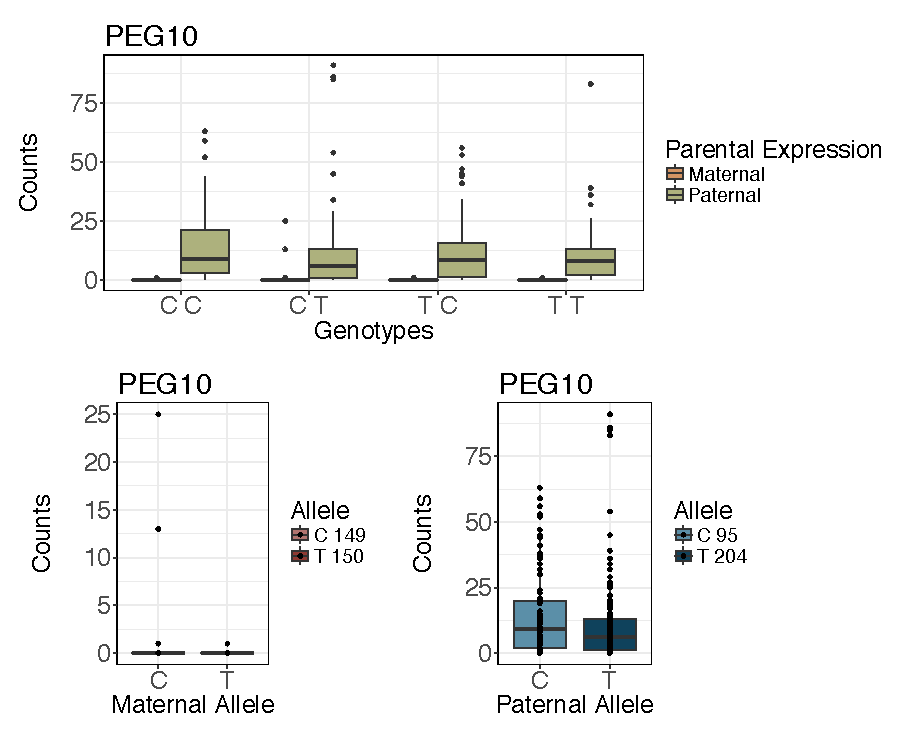
\includegraphics[width=3.5in]{img/ch04/PEG10.pdf}
\caption[Significant PO-ASE association with gene \emph{PEG10}.]{\textbf{Significant PO-ASE association with gene \emph{PEG10}.} For maternally imprinted gene \emph{PEG10} we see significant differences between maternal and paternal expression as well as paternally expression in the reciprocal heterozygotes. There is consistently less maternal expression due to the imprinting status of the gene and then more expression from the haplotype with the paternal expression with the C allele compared to the T allele in the reciprocal heterozygotes.}
\label{fig:PEG10}
\end{figure}


\subsection{Modified ASE Test on Symmetrically Expressed Genes}\label{Modified ASE Test on Symmetrically Expressed Genes} 
We were not surprised to find that the most significant genes from the PO-ASE test were imprinted genes since one haplotype of imprinted genes is silenced, and the other haplotype will be expressed contributing to the significant difference in parental gene expression. We are searching for genes that have different parental expression based on a parentally inherited allele in \emph{cis}. Imprinted genes, as those we identified in Figures \ref{fig:SNHG14}, \ref{fig:ZDBF2}, and \ref{fig:PEG10}, are consistently not expressed from the imprinted haplotype, irrespective of which allele was inherited. We wanted to identify a parent-of-origin allele effect on expression.
 
To exclude imprinted genes in the analysis we only tested genes that did not have significant asymmetrical expression (see Methods). We were searching for genes that were more symmetrically expressed from each parental haplotype to identify if a parentally inherited allele can affect expression from the same haplotype in \emph{cis}. We identified 15,340 significant SNPs (not pruned for LD) with 518 genes (using Bonferroni p-value $5.99 \times 10^{-9} $). The two most significant genes from the PO-ASE test and with symmetric expression are plotted with their most significant SNPs in Figures \ref{fig:SEC22B} and \ref{fig:ZMAT3}. The top ten genes and their most significant SNPs are listed in Table \ref{tab:poase2}.


\begin{table}[!htb]
\centering
\begin{adjustbox}{width={\textwidth}}
\begin{tabular}{@{}p{1cm}p{3cm}p{3cm}p{5cm}p{5cm}p{3cm}@{}}
 \toprule  Chr & bp & Gene & Maternal reads (Ref/Alt) & Paternal reads (Ref/Alt) & p-value \\ \midrule
1 & 404610 & SEC22B & 148/101 & 513/478 & 1.11E-98 \\
3 & 2222154 & ZMAT3 & 1320/1650 & 257/2085 & 3.53E-83\\
8 & 5425272 & PARP10 & 128/334 & 324/1018 & 1.06E-71 \\
12 & 7253839 & OAS3 & 4465/939 & 2069/4327 & 1.06E-65 \\
11 & 6368707 & IRF7 & 620/2463 & 2079/167 & 2.94E-62 \\
14 & 8008568 & IGHV2-5 & 291/295 & 22/135 & 1.80E-62 \\
17 & 8884867 & CCDC137 & 1449/865 & 173/1819 & 1.45E-57\\
14 & 7958818 & ITPK1 & 387/686 & 862/1056 & 2.48E-57\\
17 & 8865144 & SEPT9 & 560/2595 & 2594/1305 & 7.50E-50\\
17 & 8730038 & SLFN5 & 2528/3084 & 1678/2539 & 1.27E-48\\  \bottomrule
\end{tabular}
\end{adjustbox}
\caption[Top Ten Significant Genes from PO-ASE Test after Filtering Asymmetrically Expressed Genes.]{\textbf{Top Ten Significant Genes from PO-ASE Test after Filtering Asymmetrically Expressed Genes.} Filtering on symmetrical expression removed imprinted genes from being the most significant genes from PO-ASE test.}
\label{tab:poase2}
\end{table}



\begin{figure}[!htb]
\centering 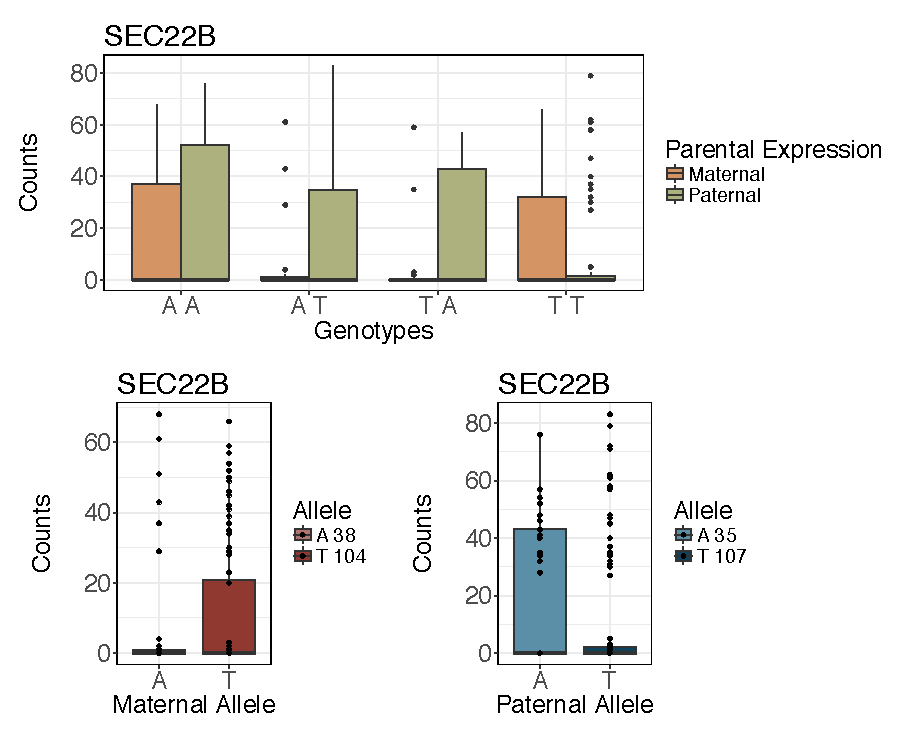
\includegraphics[width=5in]{img/ch04/SEC22B.pdf}
\caption[Significant Association from PO-ASE test with \emph{SEC22B}.]{\textbf{Significant Association from PO-ASE test with \emph{SEC22B}.} The most significant SNP (1:404610) with the most significant gene \emph{SEC22B}. In the top plot with all four genotypes we see expression from the paternal allele in all four genotypes except TT. Maternal expression is only seen in the homozygotes. In the plots by parental allele below, it is clear that the maternal T allele is associated with increased maternal expression compared to the maternal A allele at this SNP.  We see the opposite effect with paternal allele where the paternal A allele is associated with increased paternal expression and the paternal T allele with decreased expression. Based on the parental origin of the allele, the expression from the haplotype is different. }
\label{fig:SEC22B}
\end{figure}


\begin{figure}[!htb]
\centering 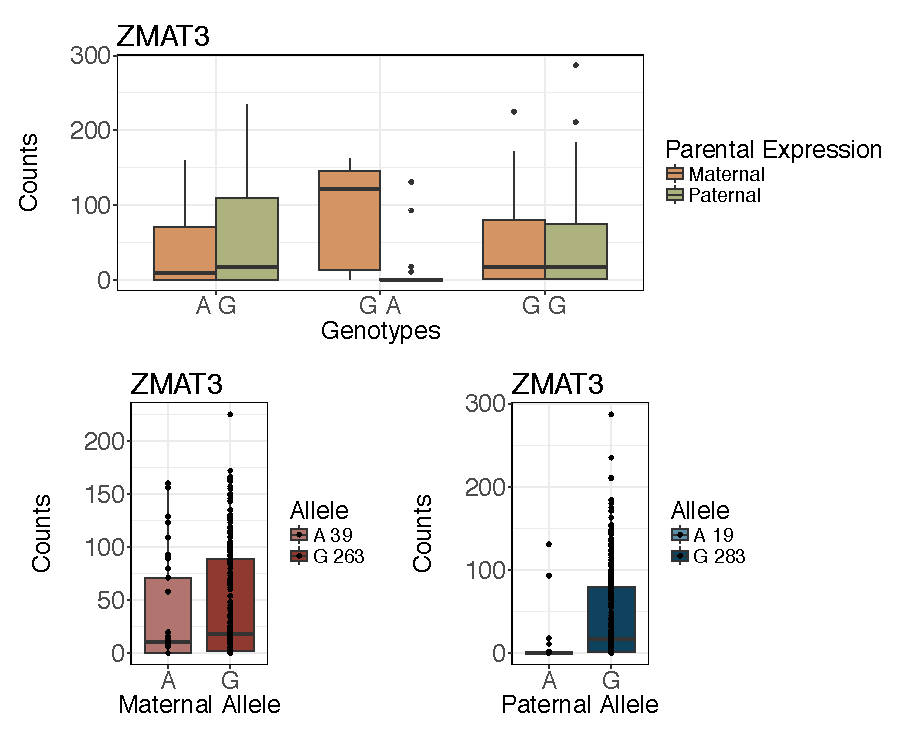
\includegraphics[width=5in]{img/ch04/ZMAT3.pdf}
\caption[Significant Association from PO-ASE test with \emph{ZMAT3}.]{\textbf{Significant Association from PO-ASE test with \emph{ZMAT3}.} The most significant SNP (3:2222154) with the second most significant gene \emph{ZMAT3}. In the top plot with all three genotypes we see expression from the paternal allele in all four genotypes except GA. Maternal expression in all genotypes. In the plots by parental allele below, it is clear that the maternal alleles are associated with maternal expression, but the paternal A allele, in contrast to the paternal G allele, is not associated with paternal expression.}
\label{fig:ZMAT3}
\end{figure}
\clearpage


\section{Discussion}\label{ch04-discussion}

Previous studies using parental alleles and gene expression have identified imprinted genes and genetic variation that affects quantitative traits \cite{Zoledziewska:2015do,Baran:2015cx,Benonisdottir:2016dz,Garg2012a}, but none to our knowledge have looked at how genetic variation can impact parent-of-origin expression from the same haplotype as the genetic variation.

Here we used parental specific gene expression in 306 Hutterites to characterize genetic effects on parental expression. We first performed a parent-of-origin opposite effect eQTL (oeQTL) test using total gene expression. We then did a maternal and a paternal eQTL study of maternal and paternal gene expression (mat-eQTL, pat-eQTL), respectively. Finally, we tested for parent-of-origin effects among reciprocal heterozygotes.

Our opposite effect model has been successful in identifying opposite effects of parentally inherited variants on quantitative traits in the Hutterites but we were not able to find any with gene expression in LCLs. These could be due to a number of reasons, including sample size and the tissue studied. LCLs are transformed cell types and the transformation could alter imprinting mechanisms. We also performed a \emph{cis} mat-eQTL and pat-eQTL study. This test identified known significant eQTLs that showed up in both the mat-eQTL and pat-eQTL results since the effect does not depend on the parent of origin. None of the variants compared across the mat-eQTL and pat-eQTL showed opposite effects by parent of origin. We were not able to find any maternal or paternally only effects on gene expression without modifying our test.

We found that most of the negative results were driven by sparsity in the data. Null expression values for gene expression could be due to two factors: 1) no heterozygous/parent-of-origin SNPs in the gene such that homozygous reads could not be assigned to a parent, or 2) there are heterozygous SNPs in the genes but there are no reads. Genes without any heterozygous SNPs for an individual were considered missing and not included in the analysis. We maintained the values for those genes for the individuals with at least one heterozygous site in a gene. Although this resulted in different numbers of individuals and genes to be tested, and provided a more conservative and informative data set, we still did not find any significant opposite effects on gene expression.

Finally, we performed a PO- ASE test among reciprocal heterozygotes to identify effects of parental variation on gene expression. The missing gene expression (i.e. uninformative) for some individuals decreased the numbers of reciprocal heterozygotes we could test for each gene.

These few results from the PO-ASE test and the opposite effect eQTL could be due to many limitations of our study. Although we were able to determine the parent of origin for many transcripts in the Hutterites, we could not assign every RNA sequencing read to a parent due to lack of heterozygous sites or missing parent-of-origin information for alleles. Missing parental gene expression resulted in very sparse data. Second, we conducted these studies in LCLs, and therefore would miss effects in other tissues or developmental time points. Additionally, our models to test for parent-of-origin eQTL effects are effective but could be much improved, such as to model over-dispersion in gene expression.

In summary, we did not identify any genetic variation with opposite parental effects on either parentally mapped gene expression or total gene expression. We did identify SNPs with parent-of-origin eQTLs even though our data are noisy and underpowered. Deeper sequencing and better modeling could potentially identify more genetic variation that impacts parental gene expression if such a biological mechanism exists. We expect these possible parent-of-origin eQTLs from the PO-ASE test to represent variation that can impact imprinting or other gene silencing mechanisms by parent of origin. For example, for the \emph{ZMAT3} gene in Figure \ref{fig:ZMAT3} we see expression from all haplotypes except from the paternal A allele. It could suggest that the paternal G allele is disrupting the mechanism that turns off paternal expression at this gene or that the paternal A allele activates a mechanism to silence the gene expression from the paternal haplotype. If more evidence for such effects are identified, it could lead to new approaches to understanding genetic variation and its impact on gene expression and, ultimately, disease and human health. 

\section{Methods}\label{ch04-methods}

\subsection{Genotypes and Sample Information}\label{Genotypes and Sample Information}
LCL RNA-seq transcripts for 306 individuals were mapped to parental haplotypes as in Chapter \ref{ch:imprinted}. We used the measures of total as well as maternal and paternal expression in this study. We used multiple approaches to characterize parent-of-origin effects on gene expression. To be conservative, we used 306 Hutterite individuals for which we have parental genotypes and tested SNPs for which we have at least three individuals in at least three of four parent-of-origin genotype classes (such that we have at least three individuals in at least one heterozygote category and one heterozygote individual will not drive our analysis). We used QCed SNPs with MAF \textgreater 5\%.

\subsection{RNA-seq QC}\label{RNA-seq QC}
Multiple approaches required different QC methods. For the total gene expression, we used normalized gene expression. First, we removed lowly expressed genes with a log count per million (cpm) greater than 1 in at least 20 individuals. The R/Bioconductor package edgeR was used to convert the RNA-seq counts to log2 TMM-normalized CPM values\cite{Robinson:2010dd,Robinson:2010cw}. Technical covariates correlated with gene expression Principal Components were regressed out (RIN, DNA concentration, RNA concentration, Flowcell/Lane). 

\subsection{Parent-of-Origin Expression QC}\label{Parent-of-Origin Expression QC}
Maternal gene expression was used as both counts and as normalized gene expression. Maternal gene expression counts were used directly from STAR gene count output\cite{Dobin:2002by} subsetted on genes included in the total gene expression analysis. 
Normalized maternal expression was calculated similar to total gene expression using edgeR and converting RNA-seq counts to log2 TMM normalized CPM values using normalization factors (library sizes) from the total gene expression (maternal gene expression too sparse on its own). The same method was used to get paternal gene expression counts and normalized paternal gene expression.

\subsection{Informative Genes}\label{Informative Genes}
To separate informative parental gene expression from uninformative parental gene expression I compiled all of the heterozygous SNPs for each individual for each gene that was expressed in LCLs. If a gene for an individual did not have any heterozygous parent-of-origin SNPs (i.e. informative SNPs), the gene was considered missing (converted to NA for downstream analysis). If there was at least one heterozygous parent-of-origin SNP in the corresponding gene, the gene expression value was not altered, since zero expression for that gene for that parent could be informative. This resulted in different numbers of genes for different individuals (Figure \ref{fig:indspergene}).

\begin{figure}[!htb]
\centering 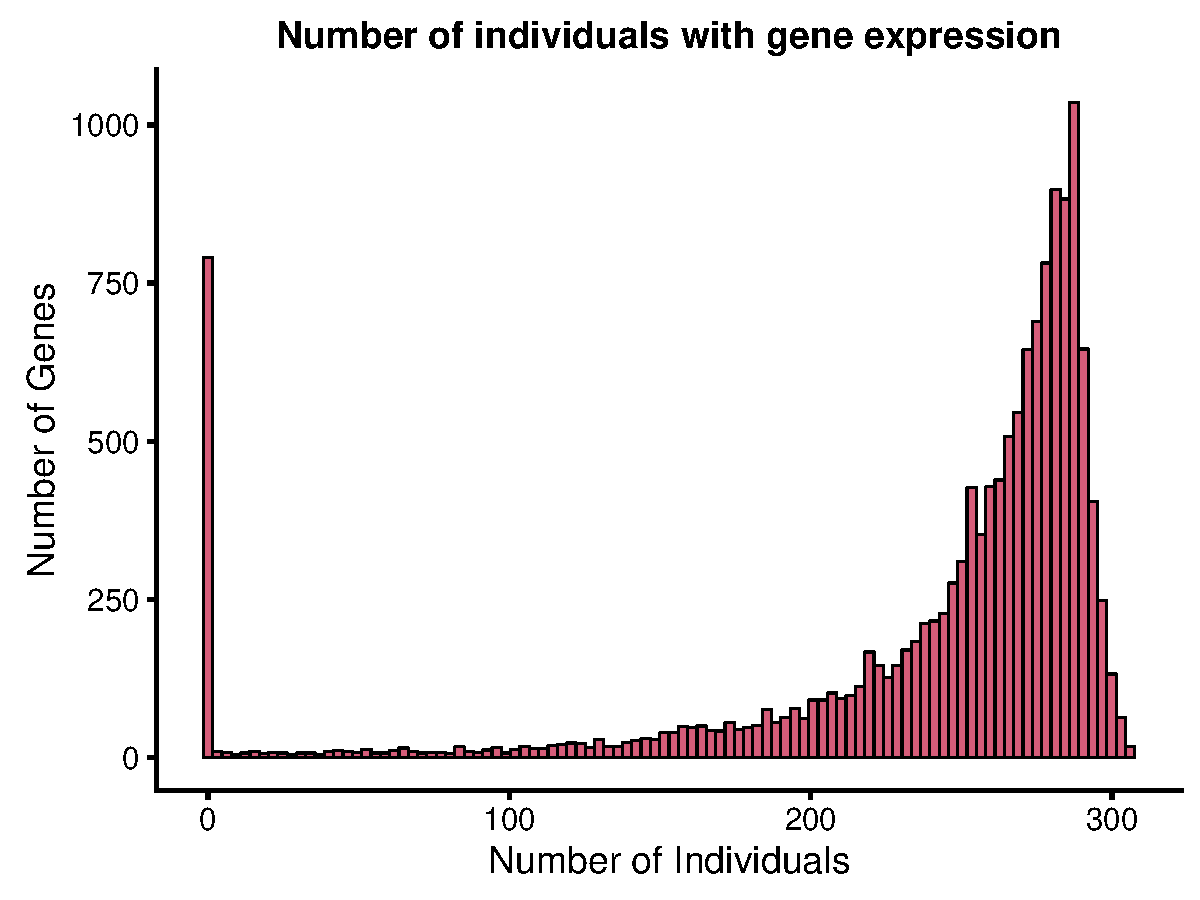
\includegraphics[width=5in]{img/ch04/fig-08-individualspergene.pdf}
\caption[Number of Individuals with Gene Expression.]{\textbf{Number of Individuals with Gene Expression.} }
\label{fig:indspergene}
\end{figure}
\clearpage


\subsection{Opposite Parent-of-Origin eQTL}\label{Opposite Parent-of-Origin eQTL}
We used the same method outlined in Chapter \ref{ch:pogwas} to detect if SNPs had opposite effects on total gene expression by parental origin. We tested SNPs in \emph{cis}, defined as +/-250kb from the TSS of the gene. The model was implemented in GEMMA\cite{Zhou2012} where we used sex and age as covariates and corrected for relatedness (see Methods from Chapter  \ref{ch:pogwas}).

\subsection{Single Parent eQTL}\label{Single Parent eQTL}
To use the parent-of-origin expression, we performed a \emph{cis} eQTL testing for specific parental effects on the same parental gene expression as follows, where  $n$ is the number of individuals, $Y_{P}$ and $Y_{M}$ are an $n \times 1$ vector of quantitative traits corresponding to paternal and maternal expression. $W$ is an $n \times c$ matrix of covariates (fixed effects) including intercept 1. $\alpha$ is a $c \times 1$ vector of covariate coefficients. $X_M$  is an $n \times 1$ vector of maternal alleles, and $X_P$ an $n \times 1$ vector of paternal alleles. $\beta_M$ and $\beta_P$ are the effect sizes of maternal and paternal alleles, respectively. g is a vector of genetic effects with $g \sim N(0, A(\sigma_g)^2 )$ where A is the genetic relatedness matrix; $\epsilon$ is a vector of non-genetic effects with $\epsilon \sim N(0,I(\sigma_e)^2)$.

\begin{equation}
Y _{M}=W\alpha + X_{M}\beta_{M}+g+\epsilon
\end{equation}

\begin{equation}
Y _{P}=W\alpha + X_{P}\beta_{P}+g+\epsilon
\end{equation}

We defined \emph{cis} as +/- 250kb from the TSS of the gene. The model was implemented in GEMMA\cite{Zhou2012} where we used sex and age as covariates and corrected for relatedness.

\subsection{PO ASE Test}\label{PO ASE Test}
We used a simple $\chi^2$ test on the reciprocal heterozygotes on their corresponding allelic expression using maternal and paternal count data corresponding to haplotype specific expression. Layout of the matrix for the test is in Table \ref{tab:chi}.

\begin{table}[!htb]
\centering
\begin{tabular}{@{}p{3cm}|p{5cm}p{5cm}@{}}
 \toprule  Genotype & C allele (ref) expression & G allele (alt) expression \\ \midrule
 $C_{M}G_{P}$ & 148  (maternal expression) & 478 (paternal expression) \\
 $G_{M}C_{P}$ & 513 (paternal expression) & 101 (maternal expression) \\
 \bottomrule
\end{tabular}
\caption[Setup for PO-ASE test.]{\textbf{Setup for PO-ASE test.} For reciprocal genotypes we use the maternal and paternal gene expression counts corresponding to opposite alleles. The chi-squared test here will determine if there is an allele and parental effect. The C and G allele in genotype refer to the reference and alternate alleles, respectively. The M and P subscript refer to maternal or paternal inherited allele.}
\label{tab:chi}
\end{table}



\subsection{Not Asymmetrically Expressed Genes}\label{Not Asymmetrically Expressed Genes}
We used a binomial test to determine which genes had more maternal expression than paternal expression. We summed paternal and maternal gene expression across all individuals for a gene and used the sum of maternal and paternal gene expression in a binomial test to determine if the ratio of maternal to the sum of maternal and paternal expression is only 1/2. We kept genes not significant (Bonferroni, p \textgreater $3.5 \times 10^{-6}$) for the Modified ASE Test. 




